\chapter{Code fundamentals}\label{chap:codefund}
To attain a higher level of localization accuracy, there are two primary goals that must be pursued.

First, the code used for underwater localization should have an auto-correlation function that approaches a Dirac impulse. This is important because it allows for more efficient detection through the use of correlation techniques.

The second factor to consider is the cross-correlation properties of the code. It is essential that these attributes meet certain criteria in order to improve separation from other sequences. Mathematically speaking, this means that the codes should be orthogonal to each other, or at least approaching orthogonality. This will be particularly useful in real-world scenarios where noise, reflections, and other artifacts may be present.
In summary, by striving to achieve both of these objectives, it is possible to significantly improve the localization accuracy.

There are a couple of techniques to generate PN sequences. Most of these methods use linear feedback shift registers to generate the codes by an initial condition or seed value. In this project I will concertize my research on gold codes, kasami codes and the basic m-sequences which are used for generating gold codes. All three code types are based on linear shift registers.

\section{Pseudo-random codes}
M-sequences are defined as binary PN codes, which are generated by linear shift registers with feedback. The sequences are periodic, and contain an equal number of zeros and ones \cite{proakis08}. 
Maximum length sequences need to fulfill certain criteria.  First its length is defined by $N=2^n - 1$ where $n$ is the maximum degree of the generator polynomial $f(X)$ \cite{sarwate80}.
 \begin{equation}
	 \lvert u\rvert=2^n-1=N,~~~\text{from polynomial}~~h(x) \text{of degree}~~n
\end{equation}
\begin{equation}
	\dfrac{N}{gcd(N,q)=N},~~~\text{from decimation polynomials}~~\widetilde{h(x)}
\end{equation}
Second the cross-correlation between m-sequences must take three values only, which are $-1$, $-t(n)$, $t(n) - 2$. With it $t(n)$ is defined by $1+2^{\lfloor0.5(n+2)\rfloor}$ \cite{sarwate80}.
If every pair of m-sequences is considered a preferred pair, they form a maximal connected set, which has a limited cardinality. Experiments conducted by Gold and Koptizke demonstrated that the number of such connected sets is limited, and that a primitive polynomial is required for an m-sequence \cite{gold65}.  

%\fignoframe{images/lfsr}{Basic structure of an LFSR (Linear Feedback Register). \cite{proakis08}}{fig:framelessFigures}

\subsection{Gold codes}
M-sequences alone may not have optimal cross-correlation properties, which can affect their orthogonality. However, when two m-sequences of the same length are combined through a modulo-2 sum, their orthogonal properties are improved. The resulting codes are known as Gold codes \cite{proakis08}.

Recent research indicates that some Gold codes have a high similarity to a Gaussian random variable, making them a suitable choice as orthogonal and pseudo-random codes \cite{merrifield}. 

\begin{equation}
Gold(u,v)=\{u,v,u\oplus v,u\oplus(v \ll1),\dots,u\oplus(v\ll N-1)\}
\end{equation}

%\fignoframe{images/gold}{LFSR structure of preferred generator polynomial of degree 13. \cite{merrifield}}{fig:framelessFigures}
\subsection{Kasami codes}

Kasami sequences are constructed in the similar fashion by using m-sequences with the exception that a second sequence, which is used in the modulo sum, is formed by decimating the default m-sequence by  $2^{m/2}$ \cite{proakis08} \cite{sarwate80} \cite{peterson72}. As a result, only one generator polynomial is needed, but this also limits the number of code variations in the set.

\begin{equation}
w=u[2^{N/2}+1]=\{u_1,\dots, u_i, \dots,u_{N}|\text{take every }i\text{-th bit of u}\} 
\end{equation}
\begin{equation}
Kasami(u)=\{u,u\oplus w,u\oplus(w \ll1),\dots,u\oplus(w\ll2^{N/2}-2)\}
\end{equation}
\section{Comparison}
For the localization process by orthogonal codes certain criteria needs to be met, which were named at the beginning of chapter \ref{chap:codefund}. To compare the before explained code types two measures are introduced.

The first one is the peak to side-lobe ratio (PSR) \ref{eq:psr}. This measure is defined by subtracting the mean from the peak of the auto-correlation. Then this value get divided by the standard deviation of the same auto-correlation. A higher PSR value signifies a lower error between the auto correlation and the perfect Dirac resulting in better detection capability. The second one is the ratio between the auto-correlation peak and the maximum of the cross-correlation (ACR) \ref{eq:acr}. A higher value indicates better code separation qualities.

The comparison is done by sampling pairs from degrees six to ten $N$ times from the set of random sequences. These pairs are then used for generating the wanted pseudo-random codes like Gold or Kasami. Afterwards for all three code types both measures are applied.  

%The last one is the correlation coefficient showing if there are similar anchros \ref{eq:coeff}, which would be a bad indicator.

\begin{equation}
PSR=\dfrac{max\{x_{ac}\}-\overline{x_{ac}}}{\sigma_{ac}}
\label{eq:psr}
\end{equation}

\begin{equation}
ACR=\dfrac{max\{x_{ac}\}}{max\{{x_{cc}\}}}
\label{eq:acr}
\end{equation}

%\begin{equation}
%\rho(a1,a2)=\dfrac{cov\{a1,a2\}}{\sigma_{a1}\cdot\sigma_{a2}}
%\label{eq:coeff}
%\end{equation}
%\begin{figure}[h]
%	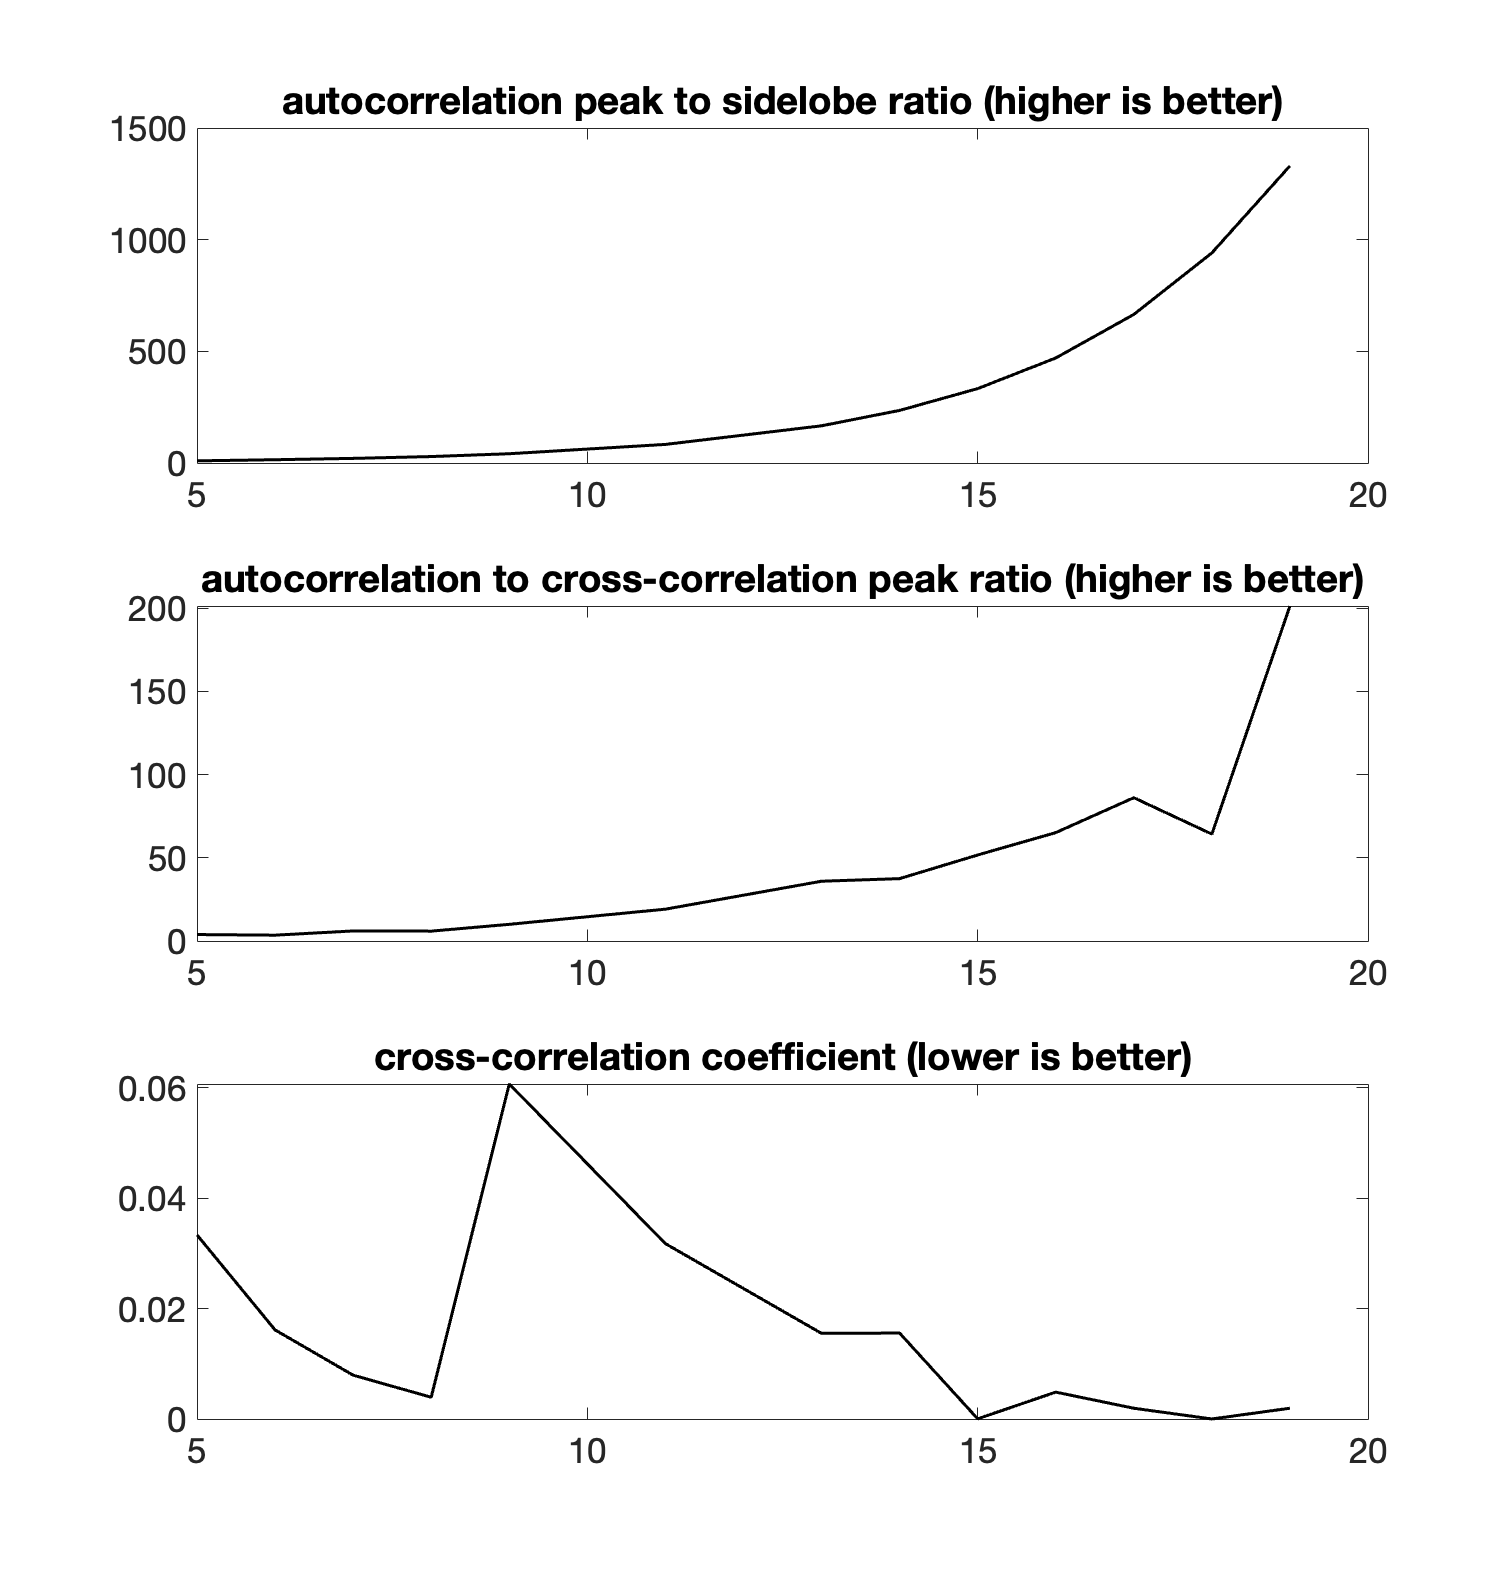
\includegraphics[width=8cm]{images/matlabplots/mseq}
%
%	\caption{Maximum Length Sequence evaluation}
%\end{figure}
%
%\begin{figure}[h]
%	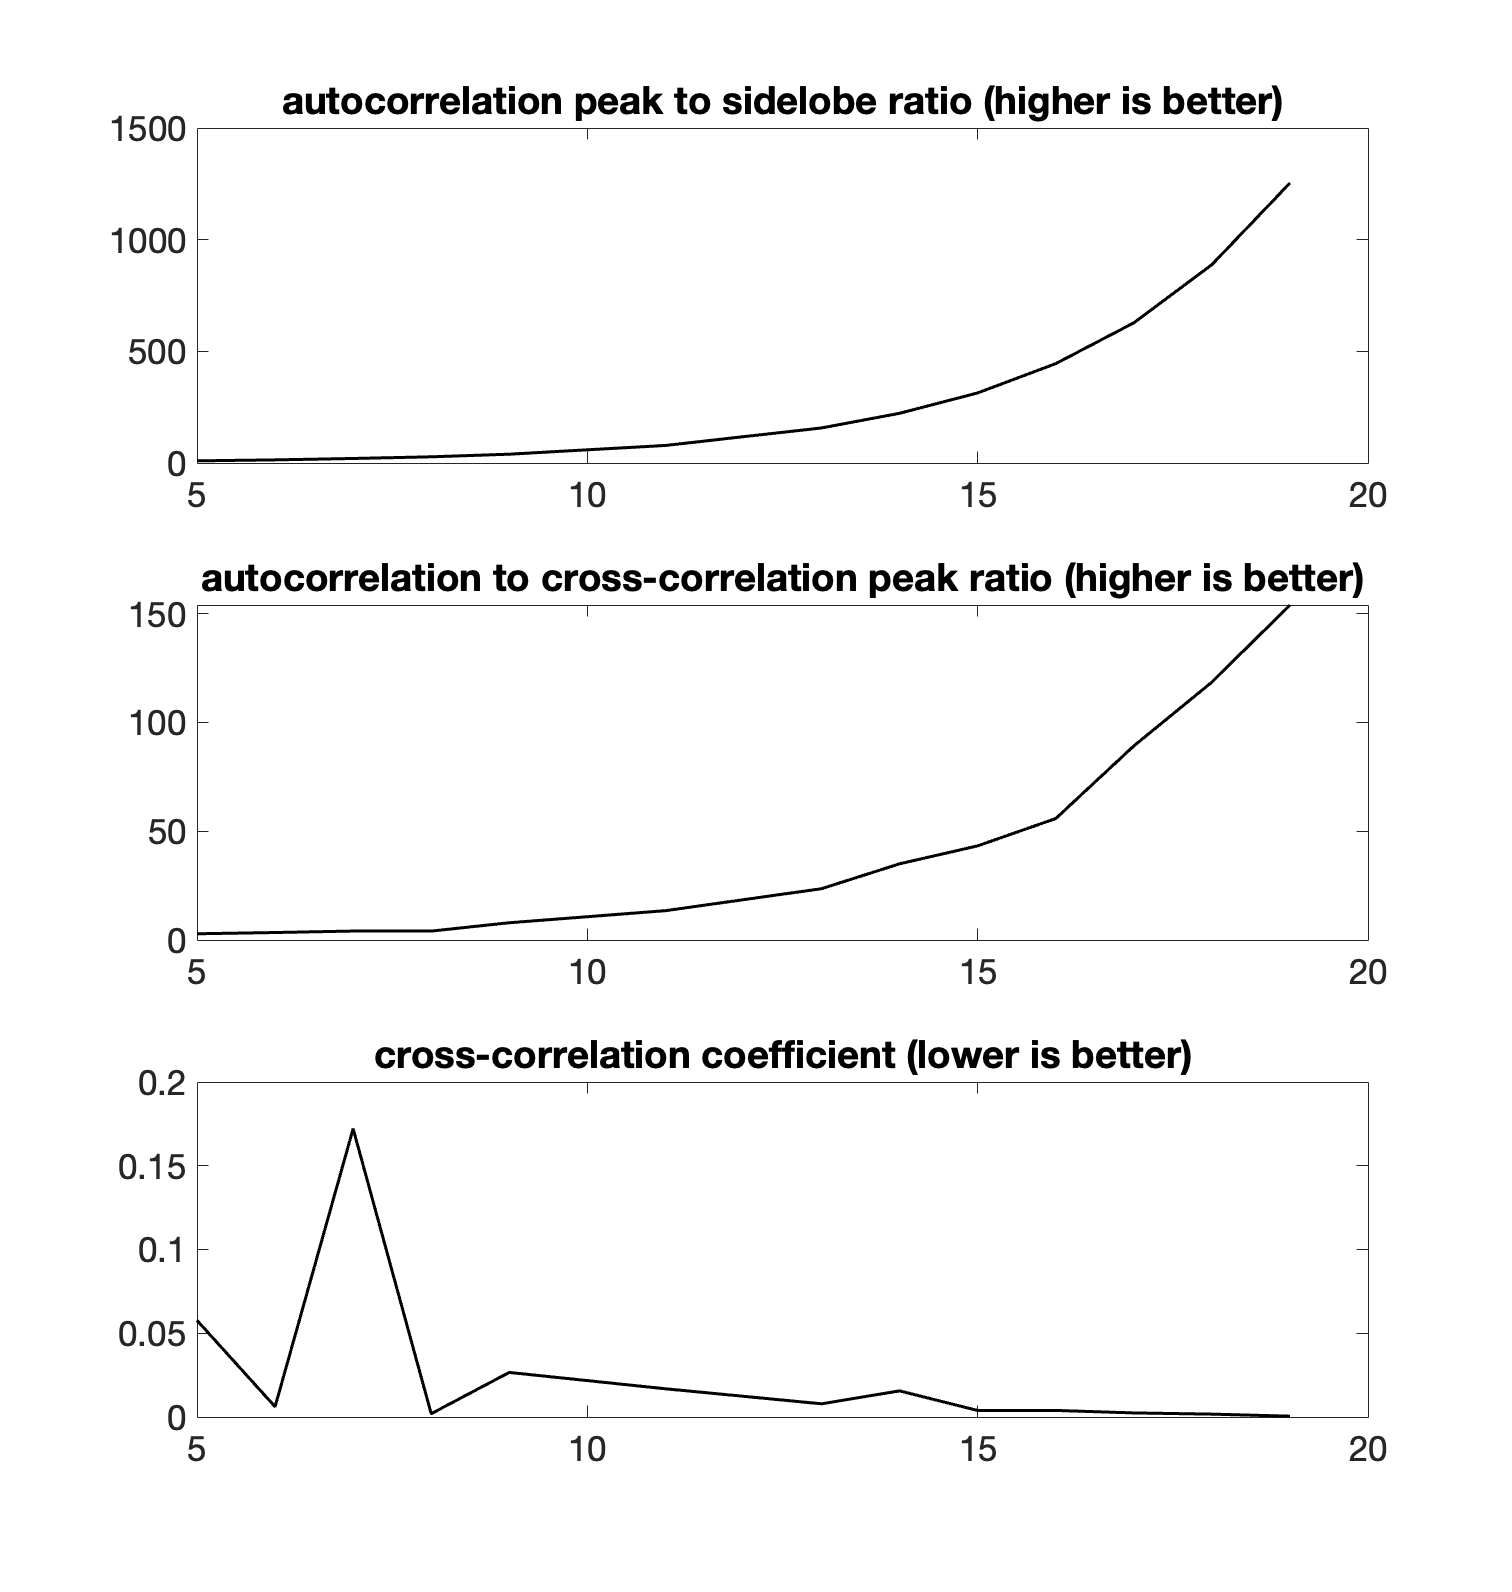
\includegraphics[width=8cm]{images/matlabplots/gold}
%
%	\caption{Gold sequence evaluation}
%\end{figure}
%
%\begin{figure}[h]
%	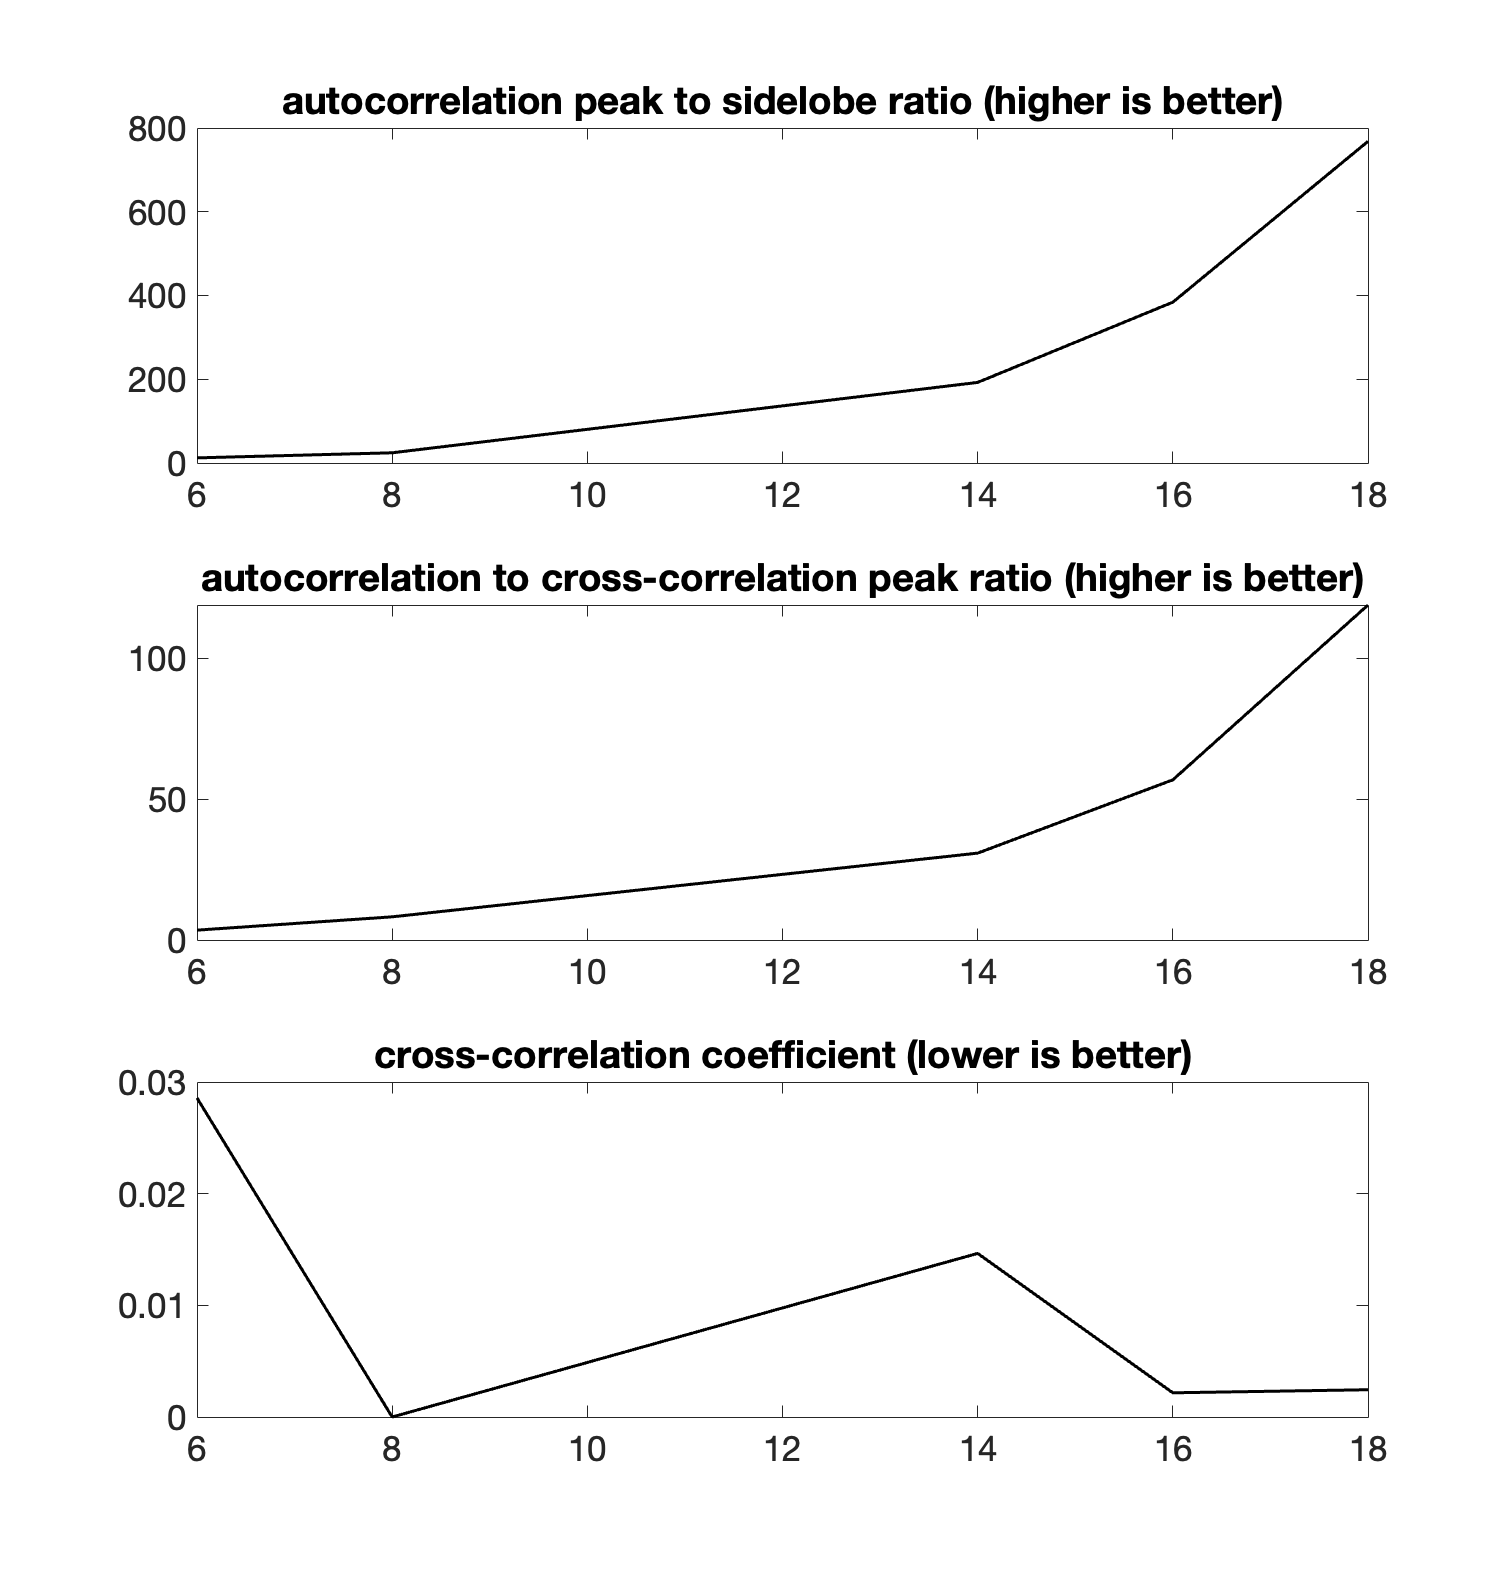
\includegraphics[width=8cm]{images/matlabplots/kasami}
%
%	\caption{Kasami sequence evaluation}
%\end{figure}
%%\fignoframe{images/matlabplots/mseq}{Basic structure of an LFSR (Linear Feedback Register). \cite{proakis08}}{fig:framelessFigures}
%%\fignoframe{images/matlabplots/gold\_10ms}{Basic structure of an LFSR (Linear Feedback Register). \cite{proakis08}}{fig:framelessFigures}
%%\fignoframe{images/matlabplots/kasami\_10ms}{Basic structure of an LFSR (Linear Feedback Register). \cite{proakis08}}{fig:framelessFigures}
%\section{Results}
In this evaluation of data, three types of codes were compared. Maximum length sequences, Gold codes, and Kasami codes. The performance of each code was assessed using two ratios, the ACR and the PSR.

From preferred polynomial all possible maximum length sequences, Gold sequences and Kasami sequences are generated. Then both measures are applied on the cross-correlation and auto-correlation functions of the random codes. The PSR and ACR measures are compared against the used polynomials. Also the best case of PSR and ACR are plotted by their given correlation function.

Maximum length sequences hold the best auto-correlation properties in comparison to its competitors. But it takes peaks in its cross-correlation, making it a rather unsuitable option for orthogonal separation. The Kasami sequence has a slight superior cross-correlation but still small peaks peeking through. The winning codes are Gold codes because of the solid auto-correlation and very fitting cross-correlation properties \ref{fig:evagoldacr}, \ref{fig:evagoldpsr}. Furthermore, Gold codes yield better scalability compared to Kasami codes, because of its larger set. Only its auto-correlations lags a bit behind its competitors but orthogonality is as much as important. 

%\begin{figure}[h]
%	\centering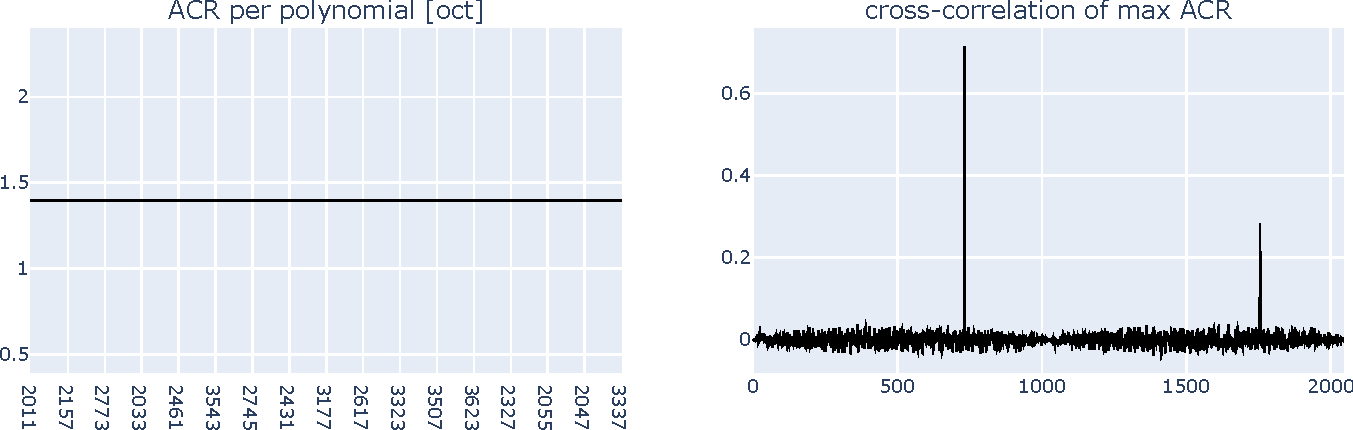
\includegraphics[width=13cm]{images/mseqevaacr}
%	
%	\caption{Evaluation of m-sequences by AC ratio}
%	\label{fig:eva}
%\end{figure}
%
%\begin{figure}[h]
%	\centering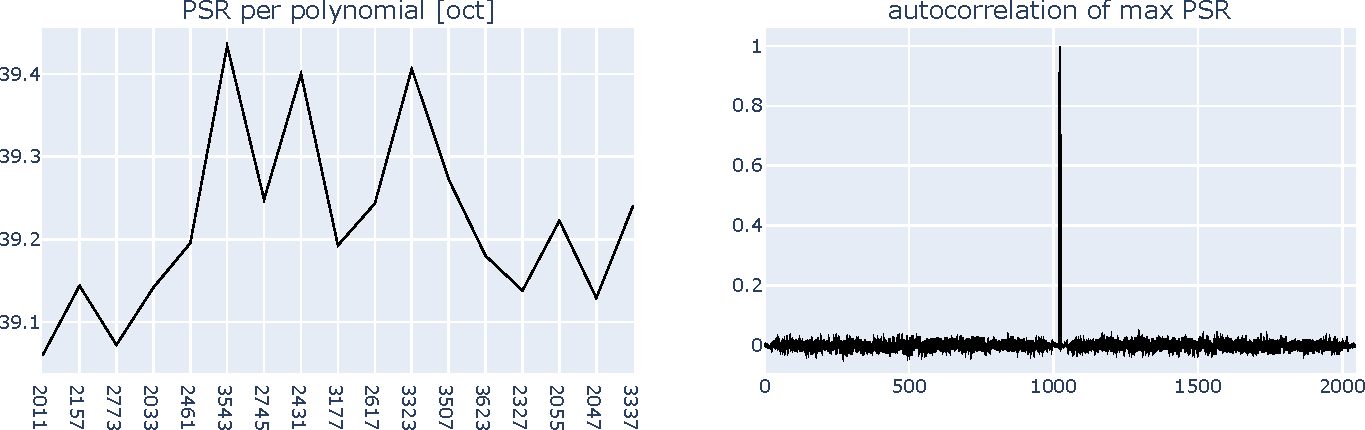
\includegraphics[width=13cm]{images/mseqevapsr}
%	
%	\caption{Evaluation of m-sequences by PS ratio}
%	\label{fig:eva}
%\end{figure}
\begin{figure}
	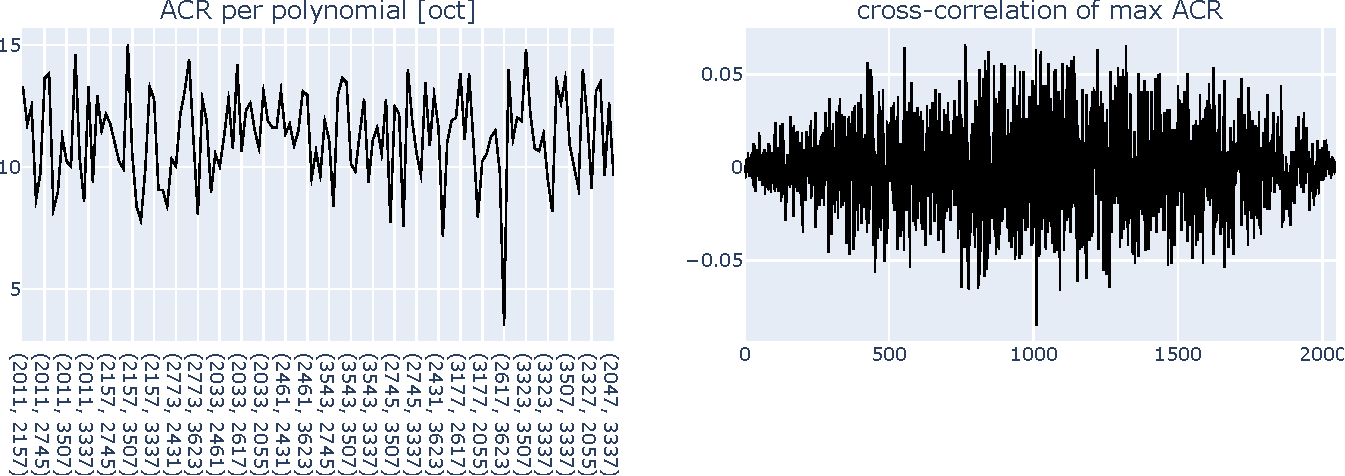
\includegraphics[width=\linewidth]{images/goldevaacr}
	\caption{Evaluation of gold sequences by AC ratio}
	\label{fig:evagoldacr}
\end{figure}
\begin{figure}
	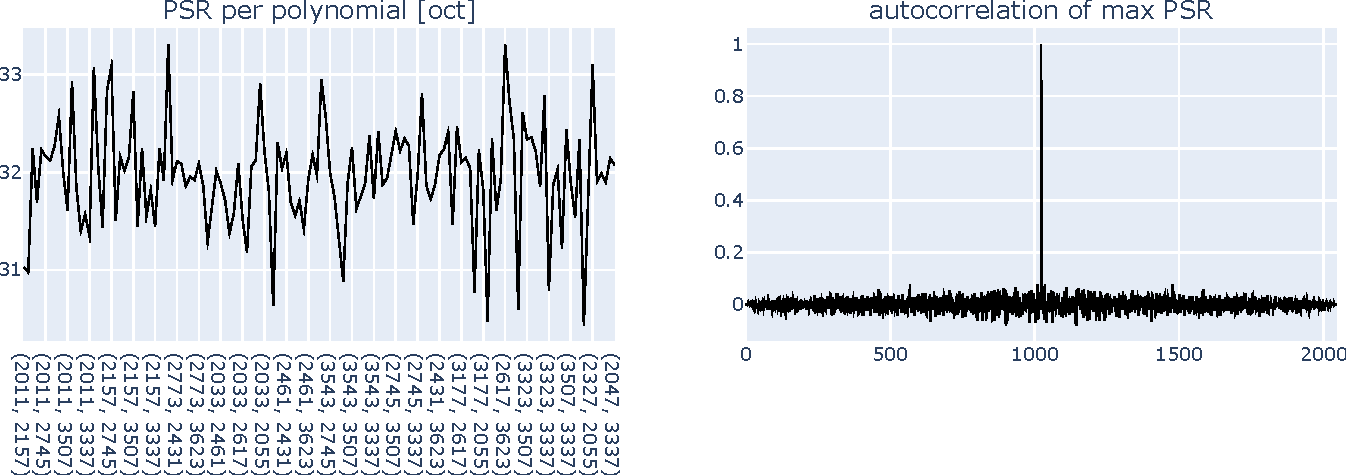
\includegraphics[width=\linewidth]{images/goldevapsr}
	\caption{Evaluation of gold sequences by PS ratio}
	\label{fig:evagoldpsr}
\end{figure}
To get more valuable data, elements from each set of codes are sampled uniformly ($N=1000$) and afterwards the evaluation parameters are applied.
The results yields that Gold codes had the least increase by PSR, but were the second best by ACR. Kasami codes were only slightly better by both PSR and ACR than Gold codes, but had a smaller set of codes available. Maximum length sequences had the highest PSR, but the worst ACR \ref{fig:eva}.

Based on these findings, it can be concluded that Gold codes are the best choice for this application. While maximum length sequences had the highest PSR, they performed poorly in terms of ACR. Gold codes, on the other hand, had a good balance of performance in both ratios, and also had a large set of codes available. In addition, Gold codes demonstrated better cross-correlated detection compared to maximum length sequences.

\begin{figure}

	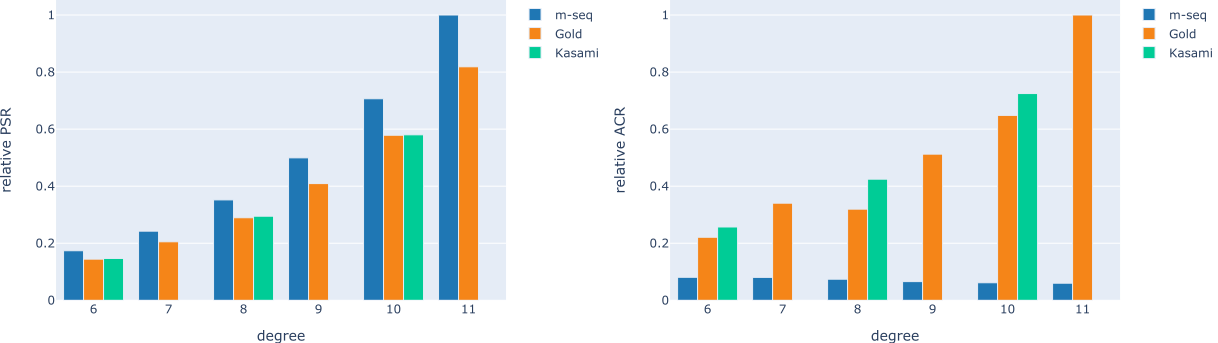
\includegraphics[width=\linewidth]{images/degCompEva}
	\caption{Evaluation by PSR and ACR for degrees 6 to 11 of all three code types}
	\label{fig:eva}
\end{figure}

%\begin{figure}[h]
%	\centering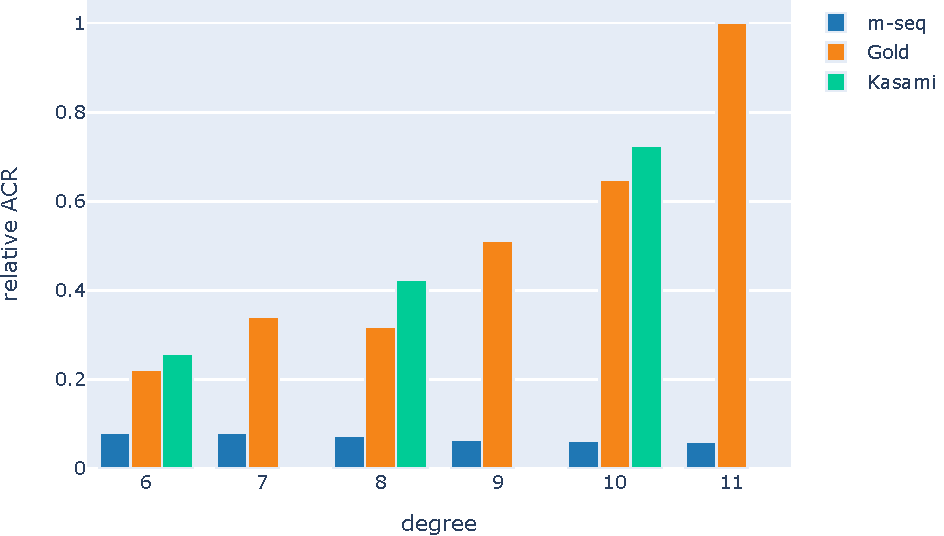
\includegraphics[width=13cm]{images/degAcrEva}
%	
%	\caption{Evaluation by relative ACR for degrees 6 to 11}
%	\label{fig:eva}
%\end{figure}
